% Select T1 before IEEEtran initializes Times, including with XeTeX/Tectonic.
\RequirePackage[T1]{fontenc}
\documentclass[conference]{IEEEtran}

% ICSPS 2026 official LaTeX template uses IEEEtran conference mode.
\usepackage{amsmath,amssymb,bm}
\usepackage{booktabs}
\usepackage{tabularx}
\usepackage{array}
\usepackage{graphicx}
% Enable bottom placement of double-column floats without changing spacing.
\usepackage{stfloats}
\usepackage{cite}
\usepackage{url}

% Keep the IEEE figure-to-text gap from stretching in sparse columns.
\setlength{\textfloatsep}{1.55\baselineskip minus 0.4\baselineskip}

\newcommand{\vect}[1]{\bm{#1}}

% Original comparison images, placed without resampling; labels remain 8 pt.
\newcommand{\comparisonpanel}[3]{%
  \begin{minipage}[t]{0.24\columnwidth}
    \centering
    \includegraphics[width=\linewidth]{#1}\par
    \vspace{2pt}%
    {\footnotesize\strut #2\par\strut #3\par}
  \end{minipage}%
}


\begin{document}

\title{SAR Despeckling via Fourier Refinement and\\
Representation-Consistent Reconstruction}

\author{\IEEEauthorblockN{Anonymous Author(s)}}

\maketitle

\begin{abstract}
The mismatch between simulated speckle and real synthetic aperture radar (SAR) observations limits the transfer of supervised restoration models. We extend the public Trans-SAR backbone with full-spectrum Fourier refinement and representation-consistent reconstruction. Residual blocks at the bottleneck and five decoder resolutions mix real and imaginary coefficients through shared real-valued channel projections. The bounded log-intensity prediction is inverted before intensity residual compensation. Masked post-adaptation then updates reconstruction on real SAR images without clean targets while freezing the inherited Transformer encoder. On 8,400 simulated pairs spanning all 21 UCMerced classes and four look numbers, one model without a look-number input achieves a macro-averaged peak signal-to-noise ratio (PSNR) of 28.14~dB and structural similarity index (SSIM) of 0.7791. PSNR is highest among the evaluated methods at every look. Removing all Fourier blocks reduces PSNR by 1.68~dB and SSIM by 0.0179. On 592 parent-disjoint real patches, adaptation lowers the M-index from 1.8213 to 1.3365 and raises the edge-preservation index from 0.4229 to 0.8214. These results establish the benefits of the evaluated reconstruction design and encoder-frozen adaptation.
\end{abstract}

\begin{IEEEkeywords}
synthetic aperture radar, despeckling, Transformer, Fourier refinement, self-supervised adaptation
\end{IEEEkeywords}

\section{Introduction}
Synthetic aperture radar (SAR) supports day-and-night observation largely independent of weather, but signal-dependent speckle obscures contrast, edges, and bright scatterers. Unit-mean Gamma noise provides a controlled multilook simulation model; focused real observations also exhibit spatial correlation, processing artifacts, and scene-dependent statistics. Despeckling must preserve scene structure under these conditions, often without clean reference images~\cite{fracastoro2021overview}.

Local statistics underpin Lee filtering~\cite{lee1980}, while SAR-BM3D exploits nonlocal recurrence using supplied noise information~\cite{parrilli2012}. CNNs learn paired image priors~\cite{chierchia2017,ko2022}; Trans-SAR and later Transformers introduce long-range interactions, multiscale reconstruction, gating, and noise guidance~\cite{perera2022,shen2025,zhang2025}. Speckle and meaningful structure nevertheless overlap in frequency, leaving an ambiguity for spatial reconstruction.

Frequency-aware networks and transformed diffusion offer alternative reconstruction representations~\cite{zhao2024,ma2024}. We combine spectral context with local features without fixed high/low bands and invert log predictions before intensity-domain fusion. To address real-data transfer, multitemporal, blind-spot, masked, and intensity-only methods relax clean-target requirements under different assumptions~\cite{dalsasso2021,molini2022,lin2025,chen2026}. Our approach uses masked self-supervision after supervised pretraining.

The contributions are threefold: (1) a public Trans-SAR extension with real--imaginary Fourier residual refinement (FDR) at the bottleneck and five decoder scales; (2) bounded log-intensity prediction followed by exact inversion and residual intensity compensation; and (3) evaluation of one model across four look numbers, with encoder-frozen masked adaptation on a real-SAR split with disjoint parent images. We explicitly identify inherited Trans-SAR components and use controlled ablations to assess the added refinement and compensation modules.

\mbox{Fig.~\ref{fig:overview}} presents the complete pipeline and separates the inherited operators from the proposed additions.
\begin{figure*}[!t]
  \centering
  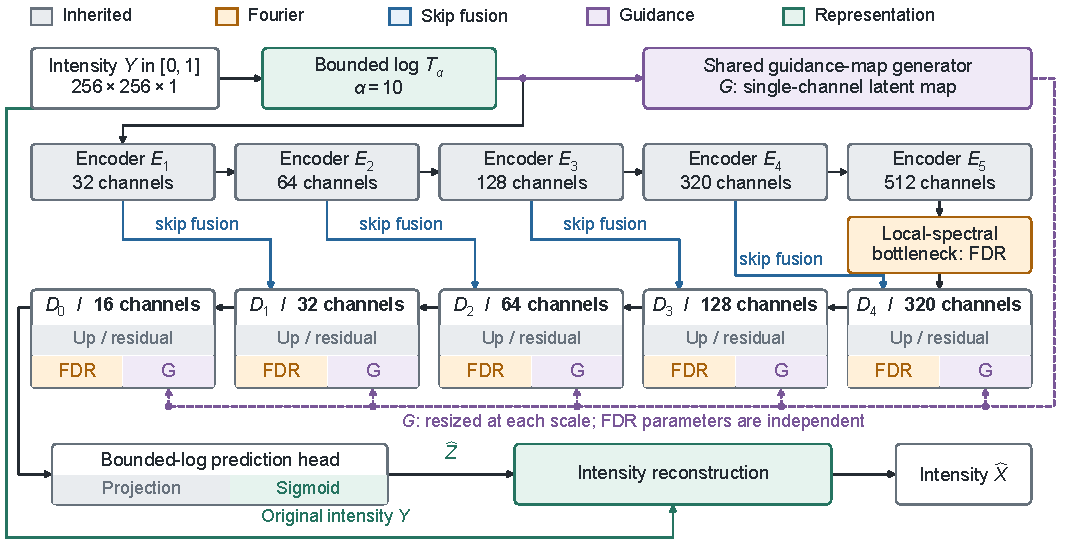
\includegraphics[width=\textwidth]{figures/fig1_overall_architecture.pdf}
  \caption{Overview of the reconstruction architecture. Gray regions denote
  inherited Trans-SAR operators; colored regions denote the added Fourier,
  skip-fusion, guidance, and representation operations. Decoder cards include
  both inherited and added components. Four encoder skips connect to the
  corresponding decoder stages. The six FDR blocks have independent parameters,
  whereas a single latent guidance map modulates all five decoder stages.
  Fig.~\ref{fig:representation_ams}(a) and (b) detail the output reconstruction
  and masked post-adaptation (AMS), respectively.}
  \label{fig:overview}
\end{figure*}

\section{Related Work}
\subsection{Model-Based and Supervised Despeckling}
Classical methods encode statistical assumptions directly: Lee filtering uses local estimates under a multiplicative-noise model~\cite{lee1980}, and SAR-BM3D combines nonlocal grouping with transform-domain shrinkage~\cite{parrilli2012}. Supervised CNNs learn from paired examples~\cite{chierchia2017}, while SAR-CAM introduces continuous multiscale attention~\cite{ko2022}. Trans-SAR pairs a five-stage spatial-reduction Transformer encoder with convolutional reconstruction~\cite{perera2022}; later systems add dynamic gates and noise-guided multiscale fusion~\cite{shen2025,zhang2025}. We build on this hierarchical framework, retaining and explicitly attributing the public Trans-SAR encoder and basic reconstruction operators.

\subsection{Frequency Processing and Image Representation}
SAR-FDD exchanges information between low- and high-frequency branches~\cite{zhao2024}; DATNet uses Fourier band decomposition with frequency-domain experts~\cite{shen2025}. Conditional diffusion with a Log-Yeo--Johnson transform instead handles multiplicative statistics through a generative formulation~\cite{ma2024}. Our refinement retains the full spectrum represented by the real fast Fourier transform (rFFT). Shared real-valued channel mixing acts on concatenated real and imaginary coefficients at each frequency coordinate, and the inverse-transformed features are fused with a local branch. At the output, the analytic inverse of the bounded log mapping restores intensity before learned compensation.

\subsection{Learning from Real SAR Observations}
Available supervision determines the assumptions for learning from real SAR. SAR2SAR uses multitemporal acquisitions~\cite{dalsasso2021}, whereas Speckle2Void couples a blind-spot likelihood with decorrelation~\cite{molini2022}. Speckle2Self combines masking with attention~\cite{lin2025}. SDS-SAR forms intensity-only pairs through correlation-aware sampling~\cite{chen2026}, and SDUDNet uses unpaired clean and noisy images~\cite{bo2025}. Following synthetic-data pretraining, our masked stage adapts reconstruction from individual noisy observations while retaining the inherited encoder parameters, providing empirical calibration to real SAR data.

\section{Proposed Method}
\subsection{Observation Model and Bounded Log Representation}
We formulate restoration in normalized linear intensity, with \(\vect{X}\) denoting the clean intensity proxy and \(\vect{Y}\) the corrupted observation. Synthetic corruption consists of independent unit-mean Gamma speckle \(\vect{N}\) with equivalent number of looks \(L\), followed by clipping:
\begin{equation}
\begin{aligned}
\vect{Y} &= \operatorname{clip}(\vect{X}\odot\vect{N},0,1),\\
N_{ij} &\sim \operatorname{Gamma}(L,L^{-1}).
\end{aligned}
\label{eq:observation}
\end{equation}
The Gamma distribution uses shape and scale parameters, giving \(\mathbb{E}[N_{ij}]=1\) and \(\operatorname{Var}(N_{ij})=L^{-1}\) before clipping. Equation~\eqref{eq:observation} defines controlled image pairs; it does not capture the full image-formation process of focused real SAR. We transform the observation with \(\alpha=10\):
\begin{equation}
T_{\alpha}(\vect{Y})=
\frac{\log(1+\alpha\vect{Y})}{\log(1+\alpha)},
\qquad \alpha=10,
\label{eq:log}
\end{equation}
with the exact inverse
\begin{equation}
T_{\alpha}^{-1}(\widehat{\vect{Z}})=
\frac{\exp[\widehat{\vect{Z}}\log(1+\alpha)]-1}{\alpha}.
\label{eq:inverse}
\end{equation}
The bounded \(\log1p\) mapping reduces the relative influence of bright scatterers and moderates the signal dependence of speckle. It does not imply that the transformed noise is additive Gaussian.

\subsection{Trans-SAR-Derived Reconstruction Path}
We retain Trans-SAR's five-stage encoder~\cite{perera2022}, overlap embeddings, spatial-reduction attention, and basic upsampling operators. From resolutions \(128^2\) to \(8^2\), channel widths are 32, 64, 128, 320, and 512; head counts are 1, 1, 2, 4, and 8; and depths are 3, 3, 4, 6, and 3. A separate guidance branch receives the same log input.

Reconstruction begins with local--spectral refinement of the deepest feature. Each decoder stage applies upsampling, skip fusion where available, FDR, residual convolution, and guidance modulation, in that order. A sigmoid head predicts bounded log intensity. Exact inversion then yields a preliminary intensity estimate, which a shallow compensator refines using the original observation.

At the bottleneck, an additional local residual wrapper surrounds the FDR block. The FDR output is summed with a separate local feature, projected, and scaled by a learnable factor initialized to 0.1 before addition to the bottleneck input. The five decoder blocks apply the same FDR mapping with independent parameters.

\subsection{Full-Spectrum Fourier Residual Refinement}
FDR couples local filtering with full-spectrum channel mixing. For input \(\vect{F}\), the spatial branch applies a depthwise \(3\times3\) convolution, a pointwise projection, and GELU. In parallel, an orthonormal two-dimensional real FFT yields \(\vect{Q}\), whose real and imaginary parts are concatenated along channels:
\begin{equation}
\begin{aligned}
\vect{Q} &= \operatorname{rFFT2}(\vect{F}),\\
\vect{Q}_{c} &= [\operatorname{Re}(\vect{Q}),
                   \operatorname{Im}(\vect{Q})].
\end{aligned}
\label{eq:fft}
\end{equation}
Two real-valued \(1\times1\) convolutions separated by GELU mix channels and real--imaginary components at each frequency coordinate. Splitting the output and applying the inverse real FFT yields \(\vect{F}_{f}\). The spatial and spectral features, \(\vect{F}_{s}\) and \(\vect{F}_{f}\), are then concatenated and projected before residual addition:
\begin{equation}
\begin{aligned}
\vect{U} &= \operatorname{GELU}
 \bigl(\vect{W}_{o,1} * [\vect{F}_{s},\vect{F}_{f}]\bigr),\\
\operatorname{FDR}(\vect{F})
 &= \vect{F}+\vect{W}_{o,2}*\vect{U}.
\end{aligned}
\label{eq:fdr}
\end{equation}
One block operates at the bottleneck; the other five act at decoder resolutions \(16^2\), \(32^2\), \(64^2\), \(128^2\), and \(256^2\). As shown in Fig.~\ref{fig:fdr}, the \(1\times1\) layers share weights across frequency coordinates while mixing channels within each coordinate. They do not couple neighboring frequencies. This operation refines the full spectrum through real--imaginary mixing without explicit band separation, magnitude--phase processing, or complex-valued convolution.
\begin{figure}[!t]
  \centering
  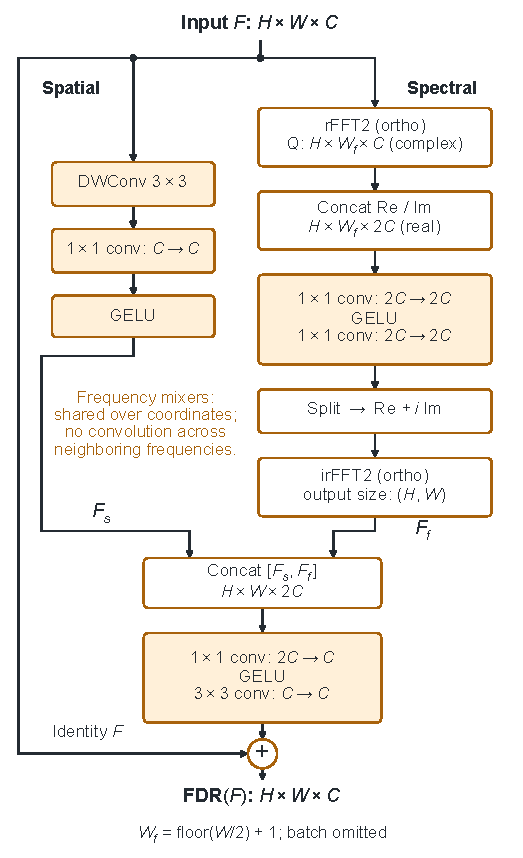
\includegraphics[width=0.94\columnwidth,trim=0 5bp 0 6bp,clip]{figures/fig2_fdr_block.pdf}
  \caption{Full-spectrum Fourier residual refinement (FDR). Local depthwise--pointwise filtering runs in parallel with spectral refinement. The one-sided rFFT contains all nonredundant frequencies. Real-valued \(1\times1\) convolutions share weights across frequency coordinates and mix the real and imaginary channels at each coordinate. An inverse rFFT restores spatial features, which are concatenated with the local features, projected, and added to the input.}
  \label{fig:fdr}
\end{figure}

\subsection{Guidance Modulation and Intensity Compensation}
The guidance branch learns a single-channel latent map from the log observation jointly with the restoration network, without dedicated noise-map or look-number targets. At each decoder scale, the resized map and feature are concatenated. Pointwise and \(3\times3\) convolutions produce a \(\tanh\) modulation, scaled by a learnable factor initialized to 0.1. Let \(\widehat{\vect{Z}}\) denote the sigmoid prediction and \(\widetilde{\vect{X}}=T_{\alpha}^{-1}(\widehat{\vect{Z}})\). A 2-to-32-to-32-to-1 compensator takes \(\vect{Y}\) and \(\widetilde{\vect{X}}\) as inputs, with \(\gamma_c\) initialized to 0.1:
\begin{equation}
\begin{aligned}
\vect{R}_{c} &= F_{\mathrm{comp}}
 ([\vect{Y},\widetilde{\vect{X}}]),\\
\widehat{\vect{X}} &= \operatorname{clip}
 (\widetilde{\vect{X}}+\gamma_c\vect{R}_{c},0,1).
\end{aligned}
\label{eq:compensation}
\end{equation}
Two \(3\times3\), 32-channel GELU layers and a single-channel residual head form the compensator. Because inversion precedes compensation, both terms added in~\eqref{eq:compensation} are in the intensity domain. The residual depends on both the observation and the preliminary restoration. The scale starts at 0.1 and remains trainable, so its initialization does not bound the correction amplitude. Final clipping constrains the output intensity, as illustrated in Fig.~\ref{fig:representation_ams}(a).



\subsection{Supervised Training and Masked Post-Adaptation}
For each \(H\times W\) image, supervised training combines mean squared intensity error with total variation regularization:
\begin{equation}
\mathcal{L}_{\mathrm{sup}}=
\frac{1}{HW}\lVert\widehat{\vect{X}}-\vect{X}\rVert_2^2
+\lambda_{\mathrm{TV}}^{\mathrm{sup}}\operatorname{TV}(\widehat{\vect{X}}).
\label{eq:supervised}
\end{equation}
TV is the sum of the mean absolute horizontal and vertical neighbor differences. The two stage-specific weights are selected on their corresponding validation splits in Section~IV-B. For masked post-adaptation (AMS), we mask each pixel independently with probability 0.2. Only masked positions contribute to the data term, with their original noisy values serving as targets:
\begin{equation}
\begin{gathered}
\vect{Y}_m=\vect{Y}\odot(1-\vect{M}),\qquad
\widehat{\vect{X}}_m=f_{\theta}(\vect{Y}_m),\\[3pt]
\mathcal{L}_{\mathrm{AMS}}=
\frac{\lVert\vect{M}\odot(\widehat{\vect{X}}_m-\vect{Y})\rVert_1}
{\max(\lVert\vect{M}\rVert_1,1)}
+\lambda_{\mathrm{AMS}}\operatorname{TV}(\widehat{\vect{X}}_m).
\end{gathered}
\label{eq:ams}
\end{equation}
AMS runs for eight epochs at a learning rate of \(10^{-6}\). We freeze the inherited Transformer encoder and update the bottleneck, decoder, guidance branch, output head, and compensator. Training masks are resampled, whereas one fixed mask per validation image keeps checkpoint selection based on the same pixel locations across epochs. Inference uses the complete unmasked observation. The masked loss does not guarantee an unbiased clean-image estimate under correlated speckle. Figure~\ref{fig:representation_ams}(b) depicts the adaptation and inference paths.

\begin{figure}[!t]
  \centering
  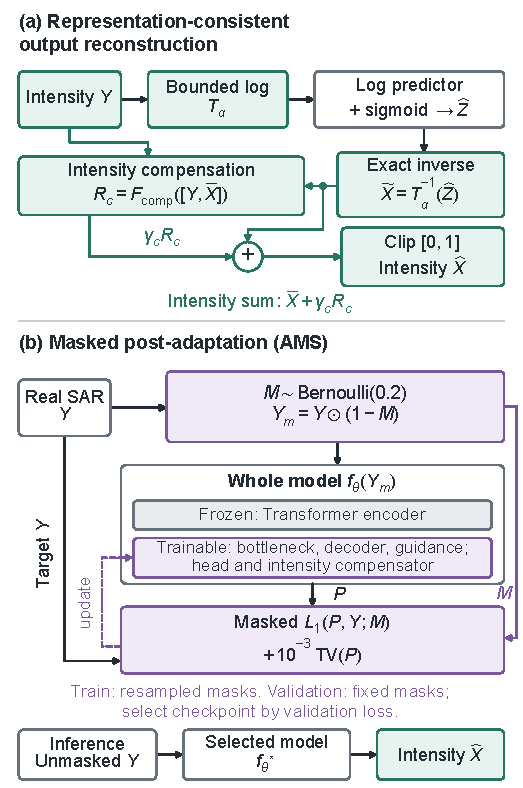
\includegraphics[width=0.98\columnwidth,trim=0 2bp 0 5bp,clip]{figures/fig3_representation_ams.pdf}
  \caption{(a) Reconstruction applies exact inversion before intensity residual
  compensation and clipping. (b) In AMS, the complete network, including the
  compensator, receives $Y_m$ in place of the generic input $Y$ in (a);
  unmasked $Y$ provides the noisy target. The Transformer encoder alone is
  frozen. Resampled training masks drive adaptation, fixed validation masks
  guide checkpoint selection, and inference uses unmasked observations.}
  \label{fig:representation_ams}
\end{figure}

% Place the wide results table with the experimental protocol.
\begin{table*}[!b]
\caption{UCM-21 Gamma-Speckle Results on 8,400 Fixed Pairs}
\label{tab:main}
\centering
\footnotesize
\setlength{\tabcolsep}{3.2pt}
\renewcommand{\arraystretch}{1.08}
\begin{tabular*}{0.86\textwidth}{@{\extracolsep{\fill}}llccccc@{}}
\toprule
\textbf{Method} & \textbf{Look mode} &
\shortstack{\(L=1\)\\PSNR / SSIM} &
\shortstack{\(L=2\)\\PSNR / SSIM} &
\shortstack{\(L=4\)\\PSNR / SSIM} &
\shortstack{\(L=8\)\\PSNR / SSIM} &
\shortstack{Macro\\PSNR / SSIM} \\
\midrule
Noisy       & --                & 12.95 / 0.2069 & 14.98 / 0.2870 & 17.37 / 0.3840 & 20.01 / 0.4916 & 16.33 / 0.3424 \\
Lee-MMSE    & oracle-\(L\)      & 21.23 / 0.5212 & 23.05 / 0.5999 & 24.71 / 0.6757 & 26.33 / 0.7455 & 23.83 / 0.6356 \\
SAR-BM3D    & oracle-\(L\)      & 25.24 / \textbf{0.7234} & 26.78 / \underline{0.7612} & \underline{28.14} / \textbf{0.7967} & 29.77 / \underline{0.8243} & 27.48 / \underline{0.7764} \\
SAR-CAM     & blind             & 22.68 / 0.5622 & 23.54 / 0.6138 & 25.89 / 0.7295 & 28.10 / 0.7949 & 25.05 / 0.6751 \\
Trans-SAR   & blind             & \underline{25.53} / 0.6446 & \underline{27.22} / 0.6963 & 28.12 / 0.7397 & \underline{29.78} / 0.7336 & \underline{27.66} / 0.7036 \\
\textbf{Ours (Full)} & blind    & \textbf{25.93} / \underline{0.7169} & \textbf{27.94} / \textbf{0.7930} & \textbf{28.57} / \underline{0.7754} & \textbf{30.13} / \textbf{0.8312} & \textbf{28.14} / \textbf{0.7791} \\
\bottomrule
\end{tabular*}
\vspace{1pt}
\parbox{0.86\textwidth}{\scriptsize PSNR is in dB. Best and second-best values among despeckling methods are bold and underlined, respectively. Oracle-\(L\) methods receive the nominal look number; blind methods do not.}
\end{table*}

\section{Experiments}
\subsection{Datasets and Evaluation Protocol}
We develop the supervised models using optical imagery from NWPU-RESISC45~\cite{cheng2017}. For each class, 20 training and 5 validation sources provide 900 and 225 independent images, respectively. RGB images are converted to grayscale, and the squared grayscale values serve as clean intensity proxies. A deterministic online schedule allocates 100,000 presentations equally to \(L\in\{1,2,4,8\}\), with 25,000 per look. Validation uses four fixed noise realizations per source, yielding 900 pairs. Paired flips and right-angle rotations provide augmentation without interpolation.

The external test set comprises all 2,100 UCMerced images from 21 classes~\cite{yang2010}. Corrupting each image once at each look produces 8,400 fixed pairs. Images not already \(256\times256\) are bilinearly resized before noise synthesis. UCMerced is excluded from model selection, so this test measures transfer between optical remote-sensing collections under simulated Gamma speckle. Noise is sampled before clipping, and no further corruption is applied.

Real-SAR evaluation uses normalized intensity patches from version~1 of Mendeley dataset fs455tz88y~\cite{vasquez2024data}. Only noisy images are used; reference images are excluded from adaptation, model selection, measurement, and visualization. The 1,469 parent images are divided into 1,175/146/148 training/validation/test parents, yielding 4,700/584/592 child patches. All four children of a \(512\times512\) parent remain in the same split. This grouping prevents overlap between parents across splits, while the evaluation remains within one data collection and does not test generalization to other regions or sensors.

All methods use identical test IDs. Unsigned 8-bit inputs are divided by 255, whereas normalized floating-point inputs are left unchanged. Per-image percentile normalization is excluded to preserve relative intensity scales.

\subsection{Implementation, Baselines, and Metrics}
Supervised training on synthetic data uses Adam, a batch size of one, an initial learning rate of \(10^{-3}\), weight decay of \(10^{-5}\), and 100,000 updates. Checkpoints are evaluated every 5,000 updates and selected by the lowest validation intensity MSE, macro-averaged by class and look. A plateau scheduler halves the learning rate with a patience of four validation events and a minimum of \(10^{-6}\).

Synthetic validation compared \(\lambda_{\mathrm{TV}}^{\mathrm{sup}}\in\{0,\allowbreak 10^{-2},\allowbreak 3\times10^{-2},\allowbreak 5\times10^{-2},\allowbreak 8\times10^{-2},\allowbreak 10^{-1}\}\) and chose \(3\times10^{-2}\), which gave the highest macro PSNR and SSIM.

\begingroup
\interlinepenalty=10000
\noindent Real-SAR validation compared \(\lambda_{\mathrm{AMS}}\in\{0,\allowbreak 10^{-4},\allowbreak 10^{-3},\allowbreak 10^{-2},\allowbreak 10^{-1}\}\) and chose \(10^{-3}\) for the best M-index/EPI tradeoff; ENL was diagnostic only. Both weights were fixed for testing.
\par
\endgroup

A single checkpoint of the proposed model handles all four \(L\) values; Ours (Full) and Ours-base both denote the configuration before real-SAR adaptation. Lee-MMSE uses a window chosen on NWPU validation. SAR-BM3D follows its square-root-input/squared-output procedure and receives the nominal \(L\); both methods are \emph{oracle-\(L\)}. SAR-CAM~\cite{ko2022}, the inherited Trans-SAR baseline~\cite{perera2022}, and our model receive only corrupted intensity. All outputs are evaluated in normalized linear intensity without display stretching.

For UCM-21, per-image PSNR and SSIM are averaged with equal weight across classes and the four looks. In the 592-patch real-SAR benchmark, five nonoverlapping \(32\times32\) regions are chosen from a fixed grid on each noisy input. Dark, zero-dominated, and saturated candidates are rejected; the remaining candidates are ranked by increasing squared coefficient of variation. The resulting 2,960 regions are fixed across methods. ENL is the mean of their ROI-level values, \(\mu^2/\sigma^2\).

Both real-SAR evaluations use the same metric definitions. The M-index combines deviations in ratio-image mean and ENL with residual structure, assessed through changes in homogeneity under random permutation; lower values indicate better performance~\cite{gomez2017}. EPI follows Eq.~(16) of~\cite{ma2024epi}: it divides the summed absolute diagonal-neighbor differences of the output by those of the noisy input. Because residual speckle can also raise EPI, we interpret it alongside ENL, M-index, and ratio-image structure~\cite{vasquez2025ratio}.

\subsection{Synthetic Comparison}
A single blind model achieves the highest PSNR point estimate at all four looks in Table~\ref{tab:main}, without an external \(L\) estimate. Its margins over the strongest competing method are 0.40, 0.72, 0.43, and 0.35~dB for \(L=1,2,4,8\), respectively. Macro performance reaches 28.14~dB/0.7791 SSIM, exceeding Trans-SAR by 0.48~dB/0.0755 and oracle-\(L\) SAR-BM3D by 0.66~dB/0.0027. SSIM rankings vary with look: SAR-BM3D leads at \(L=1,4\), whereas our method leads at \(L=2,8\).

The selected buildings scene in Fig.~\ref{fig:synthetic_qual} illustrates local restoration behavior. LEE suppresses visible fluctuations but blurs roof boundaries and small rooftop structures. SAR-BM3D, SAR-CAM, Trans-SAR, and our method preserve more roof outlines, although edge sharpness and residual texture differ. Our restoration retains the main roof contours and several rooftop structures while reducing speckle. Building outlines remain visible in its ratio image, revealing structure-related residuals and incomplete separation of scene content from speckle.

\begin{figure}[!t]
  \centering
  \begin{tabular}{@{}c@{\hspace{0.01\columnwidth}}c@{\hspace{0.01\columnwidth}}c@{\hspace{0.01\columnwidth}}c@{}}
    \comparisonpanel{figures/fig4/00_Clean.png}{(a)}{Clean} &
    \comparisonpanel{figures/fig4/01_Noisy.png}{(b)}{Noisy} &
    \comparisonpanel{figures/fig4/LEE-MMSE.png}{(c)}{LEE} &
    \comparisonpanel{figures/fig4/SAR-BM3D.png}{(d)}{SAR-BM3D} \\[3pt]
    \comparisonpanel{figures/fig4/SAR-CAM.png}{(e)}{SAR-CAM} &
    \comparisonpanel{figures/fig4/SAR-Trans.png}{(f)}{Trans-SAR} &
    \comparisonpanel{figures/fig4/Ours-base.png}{(g)}{Ours} &
    \comparisonpanel{figures/fig4/Ours-base_ratio.png}{(h)}{Ours ratio}
  \end{tabular}
  \caption{Visual comparison for a UCMerced buildings scene. LEE denotes Lee-MMSE. All panels show the same field of view in their original grayscale renderings. Panel (h) shows the ratio image for Ours and is assessed separately from the restorations.}
  \label{fig:synthetic_qual}
\end{figure}

PSNR rises from 25.93~dB at \(L=1\) to 30.13~dB at \(L=8\), whereas SSIM is nonmonotonic. Table~\ref{tab:main} reports both metrics at each look to capture this difference.

\subsection{Generalization across Three UCMerced Scene Types}
The scene-level analysis in Table~\ref{tab:ucm_scenes} supplements the full UCM-21 benchmark with 100 samples each from agricultural, buildings, and dense residential scenes at \(L=4\). These categories emphasize smooth land cover, regular boundaries, and dense texture, respectively. Their source images are excluded from supervised development. We report this fixed-look comparison separately from the four-look macro results in Table~\ref{tab:main}.

\begin{table}[!t]
\caption{Generalization on Three UCMerced Scene Types at \(L=4\)}
\label{tab:ucm_scenes}
\centering
\footnotesize
\setlength{\tabcolsep}{3.0pt}
\renewcommand{\arraystretch}{1.08}
\begin{tabular*}{\columnwidth}{@{\extracolsep{\fill}}lccc@{}}
\toprule
\textbf{Scene} & \textbf{Num.} &
\shortstack{\textbf{Noisy}\\PSNR / SSIM} &
\shortstack{\textbf{Ours-base}\\PSNR / SSIM} \\
\midrule
Agricultural & 100 & 17.7573 / 0.4218 & \textbf{29.1523 / 0.7446} \\
Buildings    & 100 & 16.6583 / 0.4625 & \textbf{27.6827 / 0.7883} \\
Dense residential & 100 & 17.5475 / 0.4557 & \textbf{30.4376 / 0.7941} \\
\midrule
Average      & 300 & 17.3211 / 0.4467 & \textbf{29.0909 / 0.7757} \\
\bottomrule
\end{tabular*}
\vspace{1pt}
\parbox{\columnwidth}{\scriptsize PSNR is in dB. All 300 samples use \(L=4\), and Average summarizes the three scene groups. Ours-base denotes the model before real-SAR adaptation. Bold values mark improvements over the noisy input.}
\end{table}

Ours-base gains 11.02--12.89~dB in PSNR and 0.3228--0.3384 in SSIM across the three categories. Mean PSNR increases from 17.3211 to 29.0909~dB, and mean SSIM from 0.4467 to 0.7757. Dense residential scenes achieve the highest restored PSNR and SSIM; buildings have the lowest PSNR, and agricultural scenes the lowest SSIM. These consistent gains demonstrate restoration across the evaluated structures at \(L=4\). The ablations below assess individual module contributions.

\subsection{Ablation Study}
Table~\ref{tab:ablation} examines the representation and compensation choices, together with the effect of removing all six Fourier blocks.
\begin{table}[!t]
\caption{Compact Ablation on UCM-21}
\label{tab:ablation}
\centering
\footnotesize
\setlength{\tabcolsep}{2.7pt}
\renewcommand{\arraystretch}{1.08}
\begin{tabularx}{\columnwidth}{@{}lXcc@{}}
\toprule
\textbf{Variant} & \textbf{Active path} & \textbf{PSNR} & \textbf{SSIM} \\
\midrule
Intensity-only & Intensity; FDR & 23.6841 & 0.6871 \\
Log-only & Log, inverse; FDR & 22.2196 & 0.7121 \\
Full w/o all FDR & Log, inverse, comp. & \underline{26.4634} & \underline{0.7612} \\
\textbf{Full} & Log, inverse, comp.; FDR & \textbf{28.1425} & \textbf{0.7791} \\
\bottomrule
\end{tabularx}
\end{table}
With all Fourier residual blocks removed, macro PSNR falls from 28.1425 to 26.4634~dB and SSIM from 0.7791 to 0.7612, a decrease of 1.6791~dB and 0.0179, respectively. The log transform, exact inverse, and intensity compensator remain active in both configurations. The difference therefore favors retaining spectral refinement within this reconstruction path.

Full outperforms Log-only by 5.9229~dB and 0.0670 SSIM, indicating a benefit from intensity compensation when FDR is present. Conversely, removing FDR tests the Fourier blocks with compensation retained. Each comparison measures a component's contribution within the tested configuration; neither quantifies the interaction between refinement and compensation.

The single-representation variants reveal a trade-off: Log-only yields lower PSNR but higher SSIM than Intensity-only. Full achieves the highest point estimates among the tested variants. Because module removal also reduces model capacity, these comparisons cannot distinguish the effect of spectral processing from that of parameter count.

\subsection{Real-SAR Adaptation}
Table~\ref{tab:real} compares all methods on 592 shared test patches drawn from 148 held-out parent images.

\begin{table}[!htbp]
\caption{No-Reference Results on 592 Real-SAR Patches}
\label{tab:real}
\centering
\footnotesize
\setlength{\tabcolsep}{3.0pt}
\renewcommand{\arraystretch}{1.08}
\begin{tabular*}{\columnwidth}{@{\extracolsep{\fill}}lrrr@{}}
\toprule
\textbf{Method} & \textbf{ENL} & \textbf{M-index}\,$\downarrow$ & \textbf{EPI}\,$\uparrow$ \\
\midrule
Noisy       & 26.25  & --                 & 1.0000 \\
SAR2SAR     & 158.39 & 2.4566             & 0.5643 \\
SDUDNet     & 83.24  & 1.7403             & 0.6786 \\
SAR-BM3D    & 25.87  & \underline{1.6579} & \underline{0.7528} \\
Trans-SAR   & 124.60 & 1.9455             & 0.5313 \\
Ours-base   & 530.85 & 1.8213             & 0.4229 \\
\textbf{Ours + AMS} & 84.72 & \textbf{1.3365} & \textbf{0.8214} \\
\bottomrule
\end{tabular*}
\vspace{1pt}
\parbox{\columnwidth}{\scriptsize\raggedright Mean ENL is reported as a smoothness diagnostic and is not ranked. For Noisy in this evaluation, M-index is undefined and EPI equals 1.0000 by identity. Bold and underlined values mark the best and second-best filtered results.}
\end{table}

Ours+AMS achieves the best M-index and EPI among the filtered outputs, followed by SAR-BM3D on both measures. Relative to Ours-base, adaptation lowers M-index from 1.8213 to 1.3365 (26.62\%) and raises EPI from 0.4229 to 0.8214 (94.23\%). ENL decreases from 530.85 to 84.72, consistent with reduced smoothing. SDUDNet has a similar ENL but a higher M-index and lower EPI, showing that comparable smoothness need not imply comparable ratio-image or edge behavior. Because training assumptions differ across methods, the direct comparison between Ours-base and Ours+AMS on identical parent-disjoint patches provides the clearest evidence of the adaptation benefit.

Reusing input-selected ROI coordinates limits method-dependent selection bias in the 592-patch evaluation. ENL still depends on regional homogeneity, so its interpretation requires the whole-image M-index, EPI, and ratio-image evidence.

The real-SAR example in Fig.~\ref{fig:real_qual} shows pronounced granular texture after SAR-BM3D, whereas SAR2SAR, SDUDNet, Trans-SAR, and Ours-base produce smoother images. Compared with Ours-base, Ours+AMS preserves clearer local boundaries and bright structures, in qualitative agreement with the aggregate increase in EPI. Its ratio image still contains structures aligned with the scene, indicating structure-related residuals. This selected example complements the dataset-level measurements in Table~\ref{tab:real}; a clean reference would be required to assess restoration fidelity directly.

\begin{figure}[!t]
  \centering
  \begin{tabular}{@{}c@{\hspace{0.01\columnwidth}}c@{\hspace{0.01\columnwidth}}c@{\hspace{0.01\columnwidth}}c@{}}
    \comparisonpanel{figures/fig5/noisy.png}{(a)}{Noisy} &
    \comparisonpanel{figures/fig5/SAR-BM3D.png}{(b)}{SAR-BM3D} &
    \comparisonpanel{figures/fig5/SAR2SAR.png}{(c)}{SAR2SAR} &
    \comparisonpanel{figures/fig5/SDUDNet.png}{(d)}{SDUDNet} \\[3pt]
    \comparisonpanel{figures/fig5/sar-trans.png}{(e)}{Trans-SAR} &
    \comparisonpanel{figures/fig5/Ours-base.png}{(f)}{Ours-base} &
    \comparisonpanel{figures/fig5/Ours-ams.png}{(g)}{Ours+AMS} &
    \comparisonpanel{figures/fig5/Ours-ams-ratio.png}{(h)}{Ours+AMS ratio}
  \end{tabular}
  \caption{Visual comparison for a real-SAR scene. Ours-base denotes the model before adaptation. The original renderings are retained, including the red inspection box in (a). Panel (h) shows the Ours+AMS ratio image, which is assessed separately from the restorations. No clean reference is shown.}
  \label{fig:real_qual}
\end{figure}

\subsection{Scene-Wise No-Reference Evaluation on Real SAR}
A complementary 60-patch real-SAR subset in Table~\ref{tab:real_scenes} contains 20 patches each from homogeneous, structural, and texture scenes. The three groups emphasize speckle suppression in uniform regions, preservation of geometric boundaries, and retention of texture, respectively. These scene-level summaries provide a separate descriptive assessment and are not pooled with the 592-patch measurements in Table~\ref{tab:real}.

% Source: ../实验结果表.md. All scene and Average entries are reproduced
% from the experimental-results table, as confirmed by the author.
\begin{table}[!t]
\caption{No-Reference Results by Real-SAR Scene Type}
\label{tab:real_scenes}
\centering
\footnotesize
\setlength{\tabcolsep}{3.0pt}
\renewcommand{\arraystretch}{1.08}
\begin{tabular*}{\columnwidth}{@{\extracolsep{\fill}}lccc@{}}
\toprule
\textbf{Model} & \textbf{ENL} & \(\mathbf{M}\)\textbf{-index}$\downarrow$ & \textbf{EPI}$\uparrow$ \\
\midrule
\multicolumn{4}{@{}l@{}}{\textit{Homogeneous: 20 patches; Noisy ENL = 32.0025}} \\
Ours-base & 740.6812 & 4.386215 & 0.312438 \\
Ours+AMS  & 88.3567  & \textbf{3.742691} & \textbf{0.818562} \\
\midrule
\multicolumn{4}{@{}l@{}}{\textit{Structural: 20 patches; Noisy ENL = 24.3142}} \\
Ours-base & 429.6054 & 0.682143 & 0.343582 \\
Ours+AMS  & 74.2189  & \textbf{0.521876} & \textbf{0.742615} \\
\midrule
\multicolumn{4}{@{}l@{}}{\textit{Texture: 20 patches; Noisy ENL = 14.9264}} \\
Ours-base & 620.8473 & 0.152604 & 0.461294 \\
Ours+AMS  & 55.6948  & \textbf{0.098531} & \textbf{0.835476} \\
\midrule
\multicolumn{4}{@{}l@{}}{\textit{Average: 60 patches; Noisy ENL = 23.7477}} \\
Ours-base & 597.0446 & 1.740321 & 0.372438 \\
Ours+AMS  & 72.7568  & \textbf{1.454366} & \textbf{0.798884} \\
\bottomrule
\end{tabular*}
\vspace{1pt}
\parbox{\columnwidth}{\scriptsize Each category uses the same 20 patches before and after AMS. Bold values mark the better M-index and EPI for each comparison. ENL is reported as a mean and is not ranked.}
% Tighten only this table's gap to the following text.
\par\vspace{-8pt}
\end{table}

The adaptation gains extend to all three scene categories. AMS lowers the M-index by 14.67\%, 23.49\%, and 35.43\% for homogeneous, structural, and texture scenes, respectively, while increasing EPI in every group. The reported Average values change from 1.740321 to 1.454366 for M-index, from 0.372438 to 0.798884 for EPI, and from 597.0446 to 72.7568 for ENL. ENL decreases relative to Ours-base in each category but remains above the noisy-input value. Together, these no-reference measurements show a consistent adaptation trend compatible with less oversmoothing and better edge retention across the evaluated scene structures.

\subsection{Limitations}
The evaluation has several limitations. Because the synthetic images originate from optical NWPU and UCM collections, they test restoration under controlled Gamma speckle without reproducing the full statistics of real SAR. The real-data split covers one collection and does not assess transfer to independent acquisitions, regions, or sensors. Masking noisy targets does not guarantee an unbiased estimate under correlated speckle, so the adaptation findings remain empirical. Parameter counts, operation counts, runtimes, and variation across initializations are not reported, leaving computational efficiency and statistical uncertainty unquantified.

Further evaluation should include independent acquisitions and paired confidence intervals that cluster UCM samples by source image and real-SAR patches by parent. These intervals should account for dependence among different looks and sibling patches. Matched training pipelines, together with model-size and runtime measurements, would permit more direct comparisons of restoration quality and computational cost.

\section{Conclusion}
We extend the public Trans-SAR backbone with Fourier refinement and representation-consistent reconstruction for SAR intensity despeckling. Six reconstruction scales apply full-spectrum real--imaginary refinement, and a bounded log estimate is analytically inverted before intensity residual compensation. On the simulated UCM-21 test, the complete model achieves the highest macro PSNR and SSIM point estimates among the compared methods. Controlled ablations show lower scores when either Fourier refinement or intensity compensation is removed. For parent-disjoint real patches, masked adaptation with a frozen encoder improves M-index and EPI while tempering the strong smoothing of the base model. Scene-level evaluations likewise show PSNR/SSIM gains in all three UCMerced categories and M-index/EPI improvements after AMS in all three real-SAR categories. These findings concern normalized single-image intensity restoration on the evaluated datasets; broader conclusions require independent real-SAR acquisitions and uncertainty analysis.

\begin{thebibliography}{00}

\bibitem{fracastoro2021overview}
G. Fracastoro \emph{et al.}, ``Deep learning methods for synthetic aperture radar image despeckling: An overview of trends and perspectives,'' \emph{IEEE Geosci. Remote Sens. Mag.}, vol.~9, no.~2, pp.~29--51, 2021, doi: 10.1109/MGRS.2021.3070956.

\bibitem{lee1980}
J.-S. Lee, ``Digital image enhancement and noise filtering by use of local statistics,'' \emph{IEEE Trans. Pattern Anal. Mach. Intell.}, vol.~PAMI-2, no.~2, pp.~165--168, 1980, doi: 10.1109/TPAMI.1980.4766994.

\bibitem{parrilli2012}
S. Parrilli, M. Poderico, C. V. Angelino, and L. Verdoliva, ``A nonlocal SAR image denoising algorithm based on LLMMSE wavelet shrinkage,'' \emph{IEEE Trans. Geosci. Remote Sens.}, vol.~50, no.~2, pp.~606--616, 2012, doi: 10.1109/TGRS.2011.2161586.

\bibitem{chierchia2017}
G. Chierchia, D. Cozzolino, G. Poggi, and L. Verdoliva, ``SAR image despeckling through convolutional neural networks,'' in \emph{Proc. IEEE IGARSS}, 2017, pp.~5438--5441, doi: 10.1109/IGARSS.2017.8128234.

\bibitem{ko2022}
J. Ko and S. Lee, ``SAR image despeckling using continuous attention module,'' \emph{IEEE J. Sel. Topics Appl. Earth Observ. Remote Sens.}, vol.~15, pp.~3--19, 2022, doi: 10.1109/JSTARS.2021.3132027.

\bibitem{perera2022}
M. V. Perera, W. G. C. Bandara, J. M. J. Valanarasu, and V. M. Patel, ``Transformer-based SAR image despeckling,'' in \emph{Proc. IEEE IGARSS}, 2022, pp.~751--754, doi: 10.1109/IGARSS46834.2022.9884596.

\bibitem{shen2025}
Y. Shen, Y. Chen, Y. Wang, L. Ma, and X. Zhang, ``DATNet: Dynamic adaptive Transformer network for SAR image denoising,'' \emph{Remote Sens.}, vol.~17, no.~17, Art. no.~3031, 2025, doi: 10.3390/rs17173031.

\bibitem{zhang2025}
L. Zhang, L. Zheng, Y. Wen, F. Zhang, F. Bo, and Y. Cen, ``Effective SAR image despeckling using noise-guided Transformer and multi-scale feature fusion,'' \emph{Remote Sens.}, vol.~17, no.~23, Art. no.~3863, 2025, doi: 10.3390/rs17233863.

\bibitem{zhao2024}
X. Zhao, F. Ren, H. Sun, and Q. Qi, ``Synthetic aperture radar image despeckling based on a deep learning network employing frequency domain decomposition,'' \emph{Electronics}, vol.~13, no.~3, Art. no.~490, 2024, doi: 10.3390/electronics13030490.

\bibitem{ma2024}
Y. Ma, P. Ke, H. Aghababaei, L. Chang, and J. Wei, ``Despeckling SAR images with Log-Yeo--Johnson transformation and conditional diffusion models,'' \emph{IEEE Trans. Geosci. Remote Sens.}, vol.~62, pp.~1--17, 2024, doi: 10.1109/TGRS.2024.3419083.

\bibitem{dalsasso2021}
E. Dalsasso, L. Denis, and F. Tupin, ``SAR2SAR: A semi-supervised despeckling algorithm for SAR images,'' \emph{IEEE J. Sel. Topics Appl. Earth Observ. Remote Sens.}, vol.~14, pp.~4321--4329, 2021, doi: 10.1109/JSTARS.2021.3071864.

\bibitem{molini2022}
A. B. Molini, D. Valsesia, G. Fracastoro, and E. Magli, ``Speckle2Void: Deep self-supervised SAR despeckling with blind-spot convolutional neural networks,'' \emph{IEEE Trans. Geosci. Remote Sens.}, vol.~60, pp.~1--17, 2022, doi: 10.1109/TGRS.2021.3065461.

\bibitem{lin2025}
H. Lin, X. Su, Z. Zeng, C. Xing, and J. Yin, ``Speckle2Self: Learning self-supervised despeckling with attention mechanism for SAR images,'' \emph{Remote Sens.}, vol.~17, no.~23, Art. no.~3840, 2025, doi: 10.3390/rs17233840.

\bibitem{chen2026}
L. Chen, Y. Yin, H. Shi, J. He, and W. Li, ``Self-supervised despeckling based solely on SAR intensity images: A general strategy,'' \emph{ISPRS J. Photogramm. Remote Sens.}, vol.~231, pp.~854--873, 2026, doi: 10.1016/j.isprsjprs.2025.11.025.

\bibitem{bo2025}
F. Bo, X. Ma, S. Hu, G. An, Y. Li, and Y. Cen, ``Speckle-driven unsupervised despeckling for SAR images,'' \emph{IEEE J. Sel. Topics Appl. Earth Observ. Remote Sens.}, vol.~18, pp.~13023--13034, 2025, doi: 10.1109/JSTARS.2025.3568854.

\bibitem{gomez2017}
L. G\'omez, R. Ospina, and A. C. Frery, ``Unassisted quantitative evaluation of despeckling filters,'' \emph{Remote Sens.}, vol.~9, no.~4, Art. no.~389, 2017, doi: 10.3390/rs9040389.

\bibitem{ma2024epi}
X. Ma, L. Li, and G. Wang, ``Blind edge-retention indicator for assessing the quality of filtered (Pol)SAR images based on a ratio gradient operator and confidence interval estimation,'' \emph{Remote Sens.}, vol.~16, no.~11, Art. no.~1992, 2024, doi: 10.3390/rs16111992.

\bibitem{vasquez2025ratio}
R. D. V\'asquez-Salazar, W. S. Puche, A. C. Frery, and L. G\'omez, ``Quality assessment of despeckling filters based on the analysis of ratio images,'' \emph{Remote Sens.}, vol.~17, no.~24, Art. no.~4048, 2025, doi: 10.3390/rs17244048.

\bibitem{cheng2017}
G. Cheng, J. Han, and X. Lu, ``Remote sensing image scene classification: Benchmark and state of the art,'' \emph{Proc. IEEE}, vol.~105, no.~10, pp.~1865--1883, 2017, doi: 10.1109/JPROC.2017.2675998.

\bibitem{yang2010}
Y. Yang and S. Newsam, ``Bag-of-visual-words and spatial extensions for land-use classification,'' in \emph{Proc. ACM SIGSPATIAL Int. Conf. Adv. Geogr. Inf. Syst.}, 2010, pp.~270--279, doi: 10.1145/1869790.1869829.

\bibitem{vasquez2024data}
R. Vasquez \emph{et al.}, ``Labeled dataset for despeckling SAR imagery,'' Mendeley Data, ver.~1, 2024, doi: 10.17632/fs455tz88y.1.

\end{thebibliography}

\end{document}
